\documentclass{article}

% Packages
\usepackage[utf8]{inputenc}
\usepackage[english]{babel}
\usepackage{amsmath}
\usepackage{latexsym}
\usepackage{amsfonts}
\usepackage[normalem]{ulem}
\usepackage{array}
\usepackage{amssymb}
\usepackage{graphicx}
\usepackage{fancyhdr}
\usepackage{siunitx}
\usepackage{algorithm}
\usepackage[noend]{algpseudocode}
\usepackage{listings}
\usepackage{float}
\usepackage[hidelinks]{hyperref}
\usepackage{caption}
\usepackage{logicproof}
\usepackage{longtable}
\usepackage{syntax}
\usepackage{lastpage}
\usepackage[a4paper,left=1in,right=1in,top=1in,bottom=1in]{geometry}
\usepackage{pdfpages}

%%% Hyperlink setup
\hypersetup {
	%linktoc = none
}

%%% Gramar environment
\setlength{\grammarparsep}{6pt plus 1pt minus 1pt} % increase separation between rules
\setlength{\grammarindent}{12em} % increase separation between LHS/RHS 
\let\syntleft\relax
\let\syntright\relax

%%% Code environment
\usepackage{listings}
\usepackage{xcolor}
\usepackage{mathpartir}
\definecolor{commentsColor}{rgb}{0.497495, 0.497587, 0.497464}
\definecolor{keywordsColor}{rgb}{0.000000, 0.000000, 0.635294}
\definecolor{stringColor}{rgb}{0.558215, 0.000000, 0.135316}

\lstset{
  	basicstyle=\ttfamily\small,                   % the size of the fonts that are used for the code
  	breakatwhitespace=false,                      % sets if automatic breaks should only happen at whitespace
  	breaklines=true,                              % sets automatic line breaking
  	frame=tb,                                     % adds a frame around the code
  	commentstyle=\color{commentsColor}\textit,    % comment style
  	keywordstyle=\color{keywordsColor}\bfseries,  % keyword style
  	stringstyle=\color{stringColor},              % string literal style
  	numbers=left,                                 % where to put the line-numbers; possible values are (none, left, right)
  	numbersep=5pt,                                % how far the line-numbers are from the code
  	numberstyle=\tiny\color{commentsColor},       % the style that is used for the line-numbers
  	showstringspaces=false,                       % underline spaces within strings only
  	tabsize=2,                                    % sets default tabsize to 2 spaces
  	language=c++
}

% Titles
\title{Å Official Documentation}
\author{The official specification for Å}
\date{}

% Page styling
\pagestyle{fancyplain}
\fancyhf{}
\renewcommand{\headrulewidth}{0pt}
\rfoot{Page \thepage \hspace{1pt} of \pageref{LastPage}}

% Custom commands
\newcommand{\newsection}[1]{
	\phantomsection
	\addcontentsline{toc}{section}{#1}
	\section*{\centering #1}
}
\newcommand{\newsubsection}[1]{
	\phantomsection
	\addcontentsline{toc}{subsection}{#1}
	\subsection*{#1}
}
\newcommand{\newsubsubsection}[1]{
	\phantomsection
	\addcontentsline{toc}{subsubsection}{#1}
	\subsubsection*{#1}
}

%% Grammar commands
\newcommand{\gtext}[1]{<$#1$>}
\newcommand{\glit}[1]{\texttt{#1}}

\begin{document}
\maketitle
\tableofcontents
\thispagestyle{empty}
\newpage
\clearpage
\setcounter{page}{1}
\pagenumbering{arabic}
\newsection{Abstract}
This document is the official document for the Å programming language. It shows how a program is parsed from source code into a binary format and then how the binary is executed. Thus this document will also contain the semantics of the language and an explanation for the default implementation of the language.  Besides explaining the semantics and syntax, this document will also explain how the source code is parsed. Additionally, how this parse result is operated on to convert it into a valid piece of Å code.
\\\\
Anything written or discussed within this document is only safely assumed to be applicable for Å version 1.0. Therefore, code and other semantics may be outdated or even too new (or features not implemented yet). This document should, therefore, only act as documentation or as guidance for the previously specified version of Å.
\newpage
\newsection{Using the Virtual Machine}
The virtual machine is first and foremost a command-line tool. It can - on Windows 10 - be run as an executable, wherein it will expect some arguments be given to it. The arguments given to the application will then be used to determine what the application will actually do.
\\\\
The machine is capable of compiling source code into Å byte code. This byte code can then be executed by the machine directly after compilation (Such that it acts as an interpreter of the source code) or be executed later. Besides compiling and executing Å code, the machine is also capable of generating a readable text version of the generated byte code. Letting the user read the result of the compilation. To add to this, the compiler can also unparse the given Abstract Syntax tree that was created during the parsing of the source code. This can help in giving the programmer a bigger insight into the interpretation of the code.
\\\\
Most arguments given to the machine can be executed in sequence (order of arguments is ignored). To which the use of the machine is simplified to simply giving it commands.
\begin{table}[H]
	\centering
	\begin{tabular}{|l|l|c|c|}
	\hline 
	Argument & Description & Mode & Version \\ \hline
	\texttt{-ga} & Generate formatted bytecode from compilation & R\textbar D & 1.0 \\ \hline
	\texttt{-lc} & Log the compile time in seconds & R\textbar D & 1.0 \\ \hline
	\texttt{-le} & Log the execute time in seconds & R\textbar D & 1.0 \\ \hline
	\texttt{-silent} & Ignores program output & R\textbar D & 1.0 \\ \hline
	\texttt{-pause} & Will need user input to close & R\textbar D & 1.0 \\ \hline
	\texttt{-trace} & Trace virtual machine operations & D & 1.0 \\ \hline
	\texttt{-test_regressive} & Run regression tests & D & 1.0 \\ \hline
	\texttt{-test_projects} & Run project regression tests & D & 1.0 \\ \hline
	\texttt{-unparse} & Unparse source after parsing & R\textbar D & 1.0 \\ \hline
	\texttt{-verify} & Verify program before running it & R\textbar D & 1.0 \\ \hline
	\texttt{-c "input file"} & Compile the input file & R\textbar D & 1.0 \\ \hline
	\texttt{-r "input file"} & Run the input file (Must be a binary) & R\textbar D & 1.0 \\ \hline
	\texttt{-o "output file"} & Output operation to file & R\textbar D & 1.0 \\ \hline
	\texttt{-oae "output file"} & Output operation to specified file and execute it & R\textbar D & 1.0 \\ \hline
	\end{tabular}
\end{table}\noindent
Some command arguments (Marked with a 'D') may only work if the VM (The \texttt{C++} code) was compiled with the \texttt{_DEBUG} flag enabled. These operations may severely hinder the performance of the language and the VM and have, therefore, been disabled for public builds. In the case of \texttt{-test_regressive}, it cannot be guaranteed the end user has the files for running the regression tests. Thus to ensure no error reports of this, or unfortunate crashes, this feature is only available for the developers of Å.
\\\\
As an example, if we wanted to compile and execute a file named "test.aa", with the code:
\begin{lstlisting}
class Program {
	Program() {
		println("Hello World from class");
	}
};

int main() {
	Program p = new Program();
	0;
};

main();
\end{lstlisting}
It could be done with the command arguments:
\begin{center}
\fbox{\texttt{call AAVM.exe -ga -unparse -c "test.aa" -oae "test.aab" -le -lc -pause}}
\end{center}
Which would give a formatted binary file ("test.aab") and an unparsed file alongside the generated binary. Additionally, we'd see the printed message in the console window, as well as the number 0.
\newpage
\newsection{Parsing}
The parsing of Å source code is split into several different stages. The first stage is the lexical analysis. Here each character of the source code is examined and, in the given context, tokenised such that the parse tree has some workable data. The parse tree is constructed by first converting the tokens into parse nodes. This constructs a flattened tree (a simple vector), that, using the syntax rules of the language are expanded. Then the more detailed parsing takes places. Lastly, the whole parse tree is converted into an abstract syntax tree (AST). Afterwards, the parsing result (the AST) is handed off to the compiler.
\\\\
The first parsing error - syntax error - recorded will stop the parsing of the code and immediately report the syntax error to the console. A short explanation of what failed (for example what was expected and what was found) is reported alongside a position (line and column) in code. If possible, a specific syntax error code is also given, hopefully, making it easier to correct or lookup solutions.
\newsubsection{Lexical Analysis}
The lexical process is rather simple and is using a two-pass system. In the first pass, most if not all words and special characters are tokenized. Each found token saves the result in a data structure containing the associated text and the position in code. The token types are shown in the table below\footnote{The $\epsilon$ character represents the whitespace character ' ' and $\Lambda$ represents the empty word - no character.}:
\begin{table}[H]
	\centering
	\begin{tabular}{|l|c|l|c|}
	\hline
	\# & Token & \centering Description	 & Regular Expression \\ \hline
	0 & invalid & Invalid Token &  \\ \hline
	1 & whitespace & Whitespace character & $\epsilon|\Lambda$ \\ \hline
	2 & identifier & Identifier - name or word & $(\underscore|[a-Z])^+([0-9]|[a-Z]|\underscore)^*$ \\ \hline
	3 & keyword & Word with specific meaning & $identifier \in \hyperref[sec:Keywords]{\textsf{keywordlist}}$ \\ \hline
	4 & separator & Separating character & $;|,|(|)|\{|\}|[|]$ \\ \hline
	5 & OP & Operator character & $+|-|*|/|\%|=|!|?|<|>|\&|||\$|\#|\textsuperscript{$\wedge$}$ \\ \hline
	6 & intlit & Integer Literal & $[1-9]^+[0-9]^*$ \\ \hline
	7 & floatlit & Floating point literal (32-bit) & $[0-9]^+.[0-9]^+\textsf{f}$ \\ \hline
	8 & doublelit & Double literal (64-bit floating point) & $[0-9]^+.[0-9]^+$ \\ \hline
	9 & charlit & Character literal & $\textsf{'}([0-9]|a-Z]|\underscore |\epsilon)\textsf{'}$ \\ \hline
	10 & stringlit & String literal & $\textsf{"}([0-9]|a-Z]|\underscore |\epsilon)^*\textsf{"}$ \\ \hline
	11 & stringOP & String operator & \\ \hline
	12 & comment & Comment token & $\textsf{//}([0-9]|[a-Z]|\underscore|\epsilon|\Lambda)^*\textsf{\textbackslash n}$ \\ \hline
	13 & accessor & Access token & $.|:$ \\ \hline
	14 & quote & Quotation token & $'|"$ \\ \hline
	\end{tabular}
\end{table} \noindent
Some of these tokens may depend on their context (For example, the keyword-identifier relation). The given regular expressions can only be used to tokenise a piece of Å source code. It should not be taken as a complete set of regular expressions defining the language.
\\\\
After the initial lexical run, the second pass starts. Here tokens that can be merged are merged. For instance, two operator tokens making up a valid operator if merged. A full list of these operators can be found in appendix 6. In this pass, string literals and char literals are also found, taking all the contents between two quote tokens and putting them into a string or char literal, depending on the length of the contents. This is part of why whitespace is tokenised, as that's how string literals keep track of the whitespace characters.
\\\\
All registered identifiers are matched against the \hyperref[sec:Keywords]{\textsf{keywordlist}}. If a match is found with any word from the above, the identifier token is "upgraded" to be a keyword token. Some keywords may be contextualised, meaning their given meaning may only apply if in the correct context. This is not decided by the lexical analysis but either by the lexical to parse tree conversion or by the parse tree formalizer (third pass of the parse tree creation algorithm).
\newpage
\newsubsection{Parse tree (PT)}
Creating the parse tree is done using a three pass algorithm. The first pass takes the result of the lexical analysis as input. It then converts the result into an array (\textsf{std::vector}) with a tree node representation of the result. This will create a flattened tree - no parents or children set. It's also here the parser determines if a token of type \texttt{OP} is a binary or a unary operation.
\\\\
The lexical token type \texttt{OP} is by default designated as a pre-unary operator, unless any literal type, end parenthesis, end index (\texttt{]}), or an identifier token is preceding it. Then it will be treated as a binary operator. If such is not the case, the operator is then treated as a pre-unary operator. Only if an identifier follows an operator (\texttt{++} and \texttt{--}) and the previous does not hold will it be defined as a post-unary operator. The partial BNF grammar for parsing this syntax would be:
\begin{grammar}
	\gtext{Expr} ::= $Expr$
	\alt \glit{(}$Expr$\glit{)}
	\alt $Expr$ $BinaryOp$ $Expr$
	\alt $PreUnaryOp$ $Expr$
	\alt $IncDecOp$ $Id$
	\alt $Id$ $IncDecOp$
	\alt \hyperref[sec:ap1]{\textsf{See full definition in Appendix 1}}

	\gtext{BinaryOp} ::= \glit{+} | \glit{-} | \glit{*} | \glit{/} | \glit{\%} | \glit{\textless} | \glit{\textgreater} | \glit{\textless}= | \glit{\textgreater}= | \glit{==} | \glit{!=} | \glit{+=} | \glit{-=} | \glit{/=} | \glit{*=} | \glit{\%=}
	\alt \glit{\textbar\textbar} | $\&\&$ | \glit{\textbar} | $\&$ | \glit{\textless\textless} | \glit{\textgreater\textgreater} | \glit{=>}
	
	\gtext{PreUnaryOp} ::= \glit{-} | \glit{!} | \glit{\#}
	
	\gtext{IncDecOp} ::= \glit{++} | \glit{--}

	\gtext{Id} ::= \hyperref[sec:ap1]{\textsf{See full definition in Appendix 1}}

\end{grammar}
\par\noindent\rule{\textwidth - 2pt}{0.2pt}\\
From the above it's not fully clear, however, post-unary operators have higher precedence than pre-unary operators. Additionally, the unary operators also have higher precedence than binary operators. Thus, the following will not be valid code:
\begin{lstlisting}
{
	int x = 5;
	int y = 5;
	x--y;
}
\end{lstlisting}
The above code will be rejected by the parser in the very first pass. The compiler will cite \textit{"'\texttt{--}' cannot be used as a binary operator"} as the reason it will not compile the above. Additionally, it should be made clear that increment and decrement operators may only operate on variables, given their \hyperref[sec:IncDecOp]{\textsf{specific behaviour}}.
\\\\
Following this token operation, the tree is unflattened. Meaning several of the syntax rules are now applied. More specifically, arithmetic, unary, assignment, groupings, and other types of bindings are applied. Meaning we here start forming the actual parse tree, such that the third pass can begin converting parts of the tree into specific node types. Which in turn will make it easier to translate into an abstract syntax tree and from there run more advanced analyses of the input - to determine the correctness of the program. No syntax errors are detected in the second pass - meaning the potential syntax errors are left to the third and final pass.
\\\\
By default this pass will attempt to find certain keywords, operators, or other patterns and create sub-expressions from this - where these sub expressions are added as children to the tree node that triggered the operation. Note, this is not where binary and unary operations (and the like) are formed. This pass is however, the pass where it's determined if something is a parameter list (for a function call or function declaration) or if it's an enclosed expression.
\newpage
The second pass follows a strict hierarchy when applying precedence rules. Which can be seen below:
 \begin{table}[H]
	\centering
	\begin{tabular}{|l|c|c|l|}
	\hline
	Priority & Name & Symbols & {\centering Description and Examples}  \\ \hline
	1 & Blocks & \texttt{\{, \}} & Code blocks - for sequences of connected statements \\ \hline
	2 & Expressions & \texttt{(, )} & Expressions, code captured between a set of parentheses \\ \hline
	3 & Indexers & \texttt{[, ]} & Indexing - or subscripting - on some identifier \\ \hline
	4 & Member Access & \texttt{::, .} & Left-to-right associative member access (\texttt{x.y} and \texttt{x::y}) \\ \hline
	5 & Unary operators & \texttt{!, \#, -, --, ++} & Examples: \texttt{!x}, \texttt{\#x}, \texttt{-x}, \texttt{--x}, \texttt{++x}, \texttt{x--}, \texttt{x++} \\ \hline
	6 & b & \texttt{\{, \}} & Code blocks - for sequences of connected statements \\ \hline
	7 &  & \texttt{\{, \}} & Code blocks - for sequences of connected statements \\ \hline
	8 &  & \texttt{\{, \}} & Code blocks - for sequences of connected statements \\ \hline
	9 &  & \texttt{\{, \}} & Code blocks - for sequences of connected statements \\ \hline
	\end{tabular}
\end{table} \noindent
\newpage
\newsubsection{Abstract Syntax Tree (AST)}
...
\newsubsubsection{Expanding the AST}
...
\newsubsubsection{Simplifying the AST}
...
\newpage
\newsection{Static Analysis}
...
\newsubsection{Type declarations}
...
\newsubsection{Function Matching}
...
\newsubsection{Building Inheritance Trees}
...
\newsubsection{Control path verification}
...
\newpage
\newsection{Type System}
...
\newsubsection{Static Type Environment}
...
\newsubsection{Dynamic Type Environment}
...
\newsubsection{Typechecking}
...
\newpage
\newsection{Evaluation of Code}
\newsubsection{Arithmetic Operators}
\label{sec:IncDecOp}
\newsubsection{Functional Operators}
\newsubsection{Declarative Operators}
\newpage
\newsection{Internals of the Virtual Machine}
...
\newsubsection{Executing bytecode}
...
\newsubsection{The operand and call stacks}
...
\newsubsection{The Ref Value Environment}
...
\newsubsection{The Garbage Collector}
\newpage
\newsection{Compiler}
...
\newsubsection{Compiling the AST}
...
\newpage
\newsubsubsection{\centering AST to Bytecode Flowchart}
\begin{figure}[H]
\centering
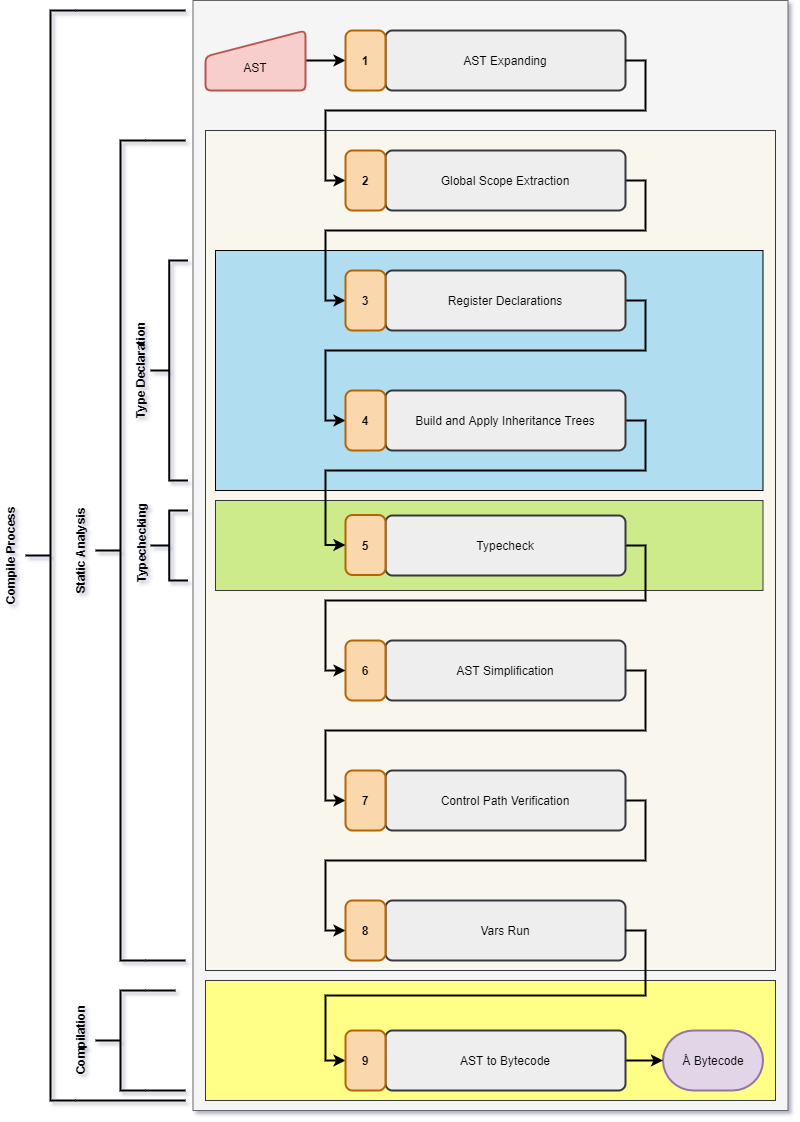
\includegraphics[width = 14cm]{CompileProcess.png}
\caption{The flowchart of the compile process}
\end{figure}\noindent
\textit{Probably some descriptive text}
\newpage
\newsubsection{Verifying Å Bytecode}
...
\newpage
\newsection{Structure of an Å-binary file}
...
\newpage
\newsection{Appendix}
The following pages are the appendices of this specification and contain full overview over the grammar, semantics, type rules, compile errors, runtime errors, and instruction list.
\newsubsection{Appendix 1: Complete Overview of Grammar}
\label{sec:ap1}
The following is a BNF grammar - extended with '$^*$' (Kleene Star)\footnote{\url{https://en.wikipedia.org/wiki/Kleene_star}} and '$^+$' (Kleene Plus). The $\epsilon$ character symbolises whitespace.
\begin{grammar}
	\gtext{Statement} ::= $Expr$\glit{;}
	\alt $Id$ \glit{=} $Expr$\glit{;} % assignment!	
	
	\gtext{Expr} := \glit{(}$Expr$\glit{)}
	\alt $Expr$ $BinaryOp$ $Expr$
	\alt $PreUnaryOp$ $Expr$
	\alt $IncDecOp$ $Id$
	\alt $Id$ $IncDecOp$
	\alt $IntLit$
	\alt $FloatLit$
	\alt $DoubleLit$
	\alt $BoolLit$
	\alt $NullLit$
	\alt $StringLit$
	\alt $CharLit$
	\alt $Id$
	
	\gtext{Decl} ::= \glit{var} $Id$ $=$ $Expr$\glit{;}
	\alt \glit{const} \glit{var} $Id$ $=$ $Expr$\glit{;}
	\alt $TypeId$ $Id$ $=$ $Expr$\glit{;}
	\alt \glit{class} $Id$ \{ $Decl^*$ \}
	\alt \glit{class} $Id$\glit{()} \{ $Decl^*$ \}
	\alt \glit{class} $Id$\glit{(}$Param$\glit{)} \{ $Decl^*$ \}
	\alt $TypeID$ $Id$\glit{()} \{ $Statement^*$ \}
	\alt \glit{void} $Id$\glit{()} \{ $Statement^*$ \}
	\alt $TypeID$ $Id$\glit{(}$Param$\glit{)} \{ $Statement^*$ \}
	\alt \glit{void} $Id$\glit{(}$Param$\glit{)} \{ $Statement^*$ \}
	
	\gtext{Param} ::= $TypeID$ $Id$ | $Param$\glit{,} $Param$
	
	\gtext{BinaryOp} ::= \glit{+} | \glit{-} | \glit{*} | \glit{/} | \glit{\%} | \glit{\textless} | \glit{\textgreater} | \glit{\textless}= | \glit{\textgreater}= | \glit{==} | \glit{!=} | \glit{+=} | \glit{-=} | \glit{/=} | \glit{*=} | \glit{\%=}
	\alt \glit{\textbar\textbar} | $\&\&$ | \glit{\textbar} | $\&$ | \glit{\textless\textless} | \glit{\textgreater\textgreater} | \glit{=>}
	
	\gtext{PreUnaryOp} ::= \glit{-} | \glit{!} | \glit{\#}
	
	\gtext{IncDecOp} ::= \glit{++} | \glit{--}

	\gtext{Digit} ::= 0 | 1 | 2 | 3 | 4 | 5 | 6 | 7 | 8 | 9

	\gtext{IntLit} ::= $Digit^+$
	
	\gtext{FloatLit} ::= $Digit^+$\glit{.}$Digit^+$\glit{f}
	
	\gtext{DoubleLit} ::= $Digit^+$\glit{.}$Digit^+$
	
\end{grammar}
\newpage
\begin{grammar}
	\gtext{BoolLit} ::= \glit{true} | \glit{false}	
	
	\gtext{NullLit} ::= \glit{null}
	
	\gtext{Letter} ::=  A | B | C | D | E | F | G
       | H | I | J | K | L | M | N
       \alt O | P | Q | R | S | T | U
       | V | W | X | Y | Z | Å 
       \alt a | b | c | d | e | f | g 
       | h | i | j | k | l | m | n 
       \alt o | p | q | r | s | t | u 
       | v | w | x | y | z | å
       
    \gtext{Id} ::= $Letter^+Digit^*Letter^*$ | \glit{_}$Id$
     
    \gtext{Character} ::= $Letter$ | $Digit$ | $\epsilon$ | \glit{_} | \glit{+} | \glit{-} | \glit{*} | \glit{/} | \glit{\%} | \glit{\#} | \glit{\textless} | \glit{\textgreater} | \glit{=} | \glit{\textbar} | \glit{\&} | \glit{\$} | \glit{€} | \glit{@} | \glit{£} | \glit{!}
    \alt \glit{?} | \glit{:} | \glit{;} | \glit{,} | \glit{.} | \glit{\^} | \glit{¨} | \glit{\~} | \glit{(} | \glit{)} | \glit{\{} | \glit{\}} | \glit{[} | \glit{]} | \glit{§} | \glit{\textbackslash n} | \glit{\textbackslash t}
       
	\gtext{StringLit} ::= \glit{\"}$Character^*$\glit{ \"}
	
	\gtext{CharLit} ::= \glit{'}$Character$\glit{'}
	
	\gtext{TypeID} ::= \glit{string} | \glit{bool} | \glit{int} | \glit{float} | \glit{char} | \glit{Any} | $Id$
	
\end{grammar}
\newpage
\newsubsection{Appendix 2: Complete Overview of Operational Semantics}
...
\begin{figure}[H]
	\centering
	\begin{mathparpagebreakable}
		\infer[Rule]
		{top}
		{bottom}
	\end{mathparpagebreakable}
\end{figure}
\newpage
\newsubsection{Appendix 3: Complete Overview of Typing Rules}
...
\newpage
\newsubsection{Appendix 4: Complete Overview of Compile Errors}
\newpage
\newsubsection{Appendix 5: Complete Overview of Instruction List}
A complete and fully up to date list can be found \underline{\href{https://github.com/JustCodiex/AA/blob/master/AAByteCode.h}{here}}.
\begin{longtable}{|l|c|c|c|c|c|c|c|}
		\hline
		\# & Opcode & Arguments & Stack before & Stack after & Description & Notes & Version \\ \hline
		0 & \texttt{NOP} & & TBD & TBD & No operation & & \textsf{V1.0} \\ \hline
		1 & \texttt{PUSHC} & & TBD & TBD & No operation & & \textsf{V1.0} \\ \hline
		2 & \texttt{PUSHN} & & TBD & TBD & No operation & & \textsf{V1.0} \\ \hline
		3 & \texttt{PUSHV} & & TBD & TBD & No operation & & \textsf{V1.0} \\ \hline
		4 & \texttt{PUSHWS} & & TBD & TBD & No operation & & \textsf{V1.0} \\ \hline
		5 & \texttt{ADD} & & TBD & TBD & No operation & & \textsf{V1.0} \\ \hline
		6 & \texttt{SUB} & & TBD & TBD & No operation & & \textsf{V1.0} \\ \hline
		7 & \texttt{MUL} & & TBD & TBD & No operation & & \textsf{V1.0} \\ \hline
		8 & \texttt{DIV} & & TBD & TBD & No operation & & \textsf{V1.0} \\ \hline
		9 & \texttt{MOD} & & TBD & TBD & No operation & & \textsf{V1.0} \\ \hline
		10 & \texttt{NNEG} & & TBD & TBD & No operation & & \textsf{V1.0} \\ \hline
		11 & \texttt{CONCAT} & & TBD & TBD & No operation & & \textsf{V1.0} \\ \hline
		12 & \texttt{LEN} & & TBD & TBD & No operation & & \textsf{V1.0} \\ \hline
		13 & \texttt{INC} & & TBD & TBD & No operation & & \textsf{V1.0} \\ \hline
		14 & \texttt{DEC} & & TBD & TBD & No operation & & \textsf{V1.0} \\ \hline
		15 & \texttt{SETVAR} & & TBD & TBD & No operation & & \textsf{V1.0} \\ \hline
		16 & \texttt{GETVAR} & & TBD & TBD & No operation & & \textsf{V1.0} \\ \hline
		17 & \texttt{SETFIELD} & & TBD & TBD & No operation & & \textsf{V1.0} \\ \hline
		18 & \texttt{GETFIELD} & & TBD & TBD & No operation & & \textsf{V1.0} \\ \hline
		19 & \texttt{GETELEM} & & TBD & TBD & No operation & & \textsf{V1.0} \\ \hline
		20 & \texttt{SETELEM} & & TBD & TBD & No operation & & \textsf{V1.0} \\ \hline
		21 & \texttt{JMP} & & TBD & TBD & No operation & & \textsf{V1.0} \\ \hline
		22 & \texttt{JMPF} & & TBD & TBD & No operation & & \textsf{V1.0} \\ \hline
		23 & \texttt{JMPT} & & TBD & TBD & No operation & & \textsf{V1.0} \\ \hline
		24 & \texttt{LJMP} & & TBD & TBD & No operation & Not used & \textsf{V1.0} \\ \hline
		25 & \texttt{CALL} & & TBD & TBD & No operation & & \textsf{V1.0} \\ \hline
		26 & \texttt{VCALL} & & TBD & TBD & No operation & & \textsf{V1.0} \\ \hline
		27 & \texttt{XCALL} & & TBD & TBD & No operation & & \textsf{V1.0} \\ \hline
		28 & \texttt{RET} & & TBD & TBD & No operation & & \textsf{V1.0} \\ \hline
		29 & \texttt{CMPE} & & TBD & TBD & No operation & & \textsf{V1.0} \\ \hline
		30 & \texttt{CMPNE} & & TBD & TBD & No operation & & \textsf{V1.0} \\ \hline
		31 & \texttt{LE} & & TBD & TBD & No operation & & \textsf{V1.0} \\ \hline
		32 & \texttt{GE} & & TBD & TBD & No operation & & \textsf{V1.0} \\ \hline
		33 & \texttt{GEQ} & & TBD & TBD & No operation & & \textsf{V1.0} \\ \hline
		34 & \texttt{LEQ} & & TBD & TBD & No operation & & \textsf{V1.0} \\ \hline
		35 & \texttt{LNEG} & & TBD & TBD & No operation & & \textsf{V1.0} \\ \hline
		36 & \texttt{LAND} & & TBD & TBD & No operation & & \textsf{V1.0} \\ \hline
		37 & \texttt{LOR} & & TBD & TBD & No operation & & \textsf{V1.0} \\ \hline
		38 & \texttt{BAND} & & TBD & TBD & No operation & & \textsf{V1.0} \\ \hline
		39 & \texttt{BOR} & & TBD & TBD & No operation & & \textsf{V1.0} \\ \hline
		40 & \texttt{TUPLECMP} & & TBD & TBD & No operation & & \textsf{V1.0} \\ \hline
		41 & \texttt{TUPLENEW} & & TBD & TBD & No operation & & \textsf{V1.0} \\ \hline
		42 & \texttt{TUPLEGET} & & TBD & TBD & No operation & & \textsf{V1.0} \\ \hline
		43 & \texttt{ALLOC} & & TBD & TBD & No operation & Not used & \textsf{V1.0} \\ \hline
		44 & \texttt{ALLOCARRAY} & & TBD & TBD & No operation & & \textsf{V1.0} \\ \hline
		45 & \texttt{CTOR} & & TBD & TBD & No operation & & \textsf{V1.0} \\ \hline
		46 & \texttt{TRY} & & TBD & TBD & No operation & & \textsf{V1.0} \\ \hline
		47 & \texttt{THROW} & & TBD & TBD & No operation & & \textsf{V1.0} \\ \hline
		48 & \texttt{BRK} & & TBD & TBD & No operation & & \textsf{V1.0} \\ \hline
		49 & \texttt{POP} & & TBD & TBD & No operation & & \textsf{V1.0} \\ \hline
		50 & \texttt{CASTI2F} & & TBD & TBD & No operation & & \textsf{V1.0} \\ \hline
		51 & \texttt{CASTF2I} & & TBD & TBD & No operation & & \textsf{V1.0} \\ \hline
		52 & \texttt{CASTF2I} & & TBD & TBD & No operation & & \textsf{V1.0} \\ \hline
		53 & \texttt{CASTS2F} & & TBD & TBD & No operation & & \textsf{V1.0} \\ \hline
		54 & \texttt{CASTF2S} & & TBD & TBD & No operation & & \textsf{V1.0} \\ \hline
		55 & \texttt{CASTL2F} & & TBD & TBD & No operation & & \textsf{V1.0} \\ \hline
		56 & \texttt{CASTL2I} & & TBD & TBD & No operation & & \textsf{V1.0} \\ \hline
		57 & \texttt{CASTL2S} & & TBD & TBD & No operation & & \textsf{V1.0} \\ \hline
		58 & \texttt{CASTF2L} & & TBD & TBD & No operation & & \textsf{V1.0} \\ \hline
		59 & \texttt{CASTI2D} & & TBD & TBD & No operation & & \textsf{V1.0} \\ \hline
		60 & \texttt{CASTS2D} & & TBD & TBD & No operation & & \textsf{V1.0} \\ \hline
		61 & \texttt{CASTF2D} & & TBD & TBD & No operation & & \textsf{V1.0} \\ \hline
		62 & \texttt{CASTL2D} & & TBD & TBD & No operation & & \textsf{V1.0} \\ \hline
		63 & \texttt{CASTD2I} & & TBD & TBD & No operation & & \textsf{V1.0} \\ \hline
		64 & \texttt{CASTD2S} & & TBD & TBD & No operation & & \textsf{V1.0} \\ \hline
		65 & \texttt{CASTD2F} & & TBD & TBD & No operation & & \textsf{V1.0} \\ \hline
		66 & \texttt{CASTD2L} & & TBD & TBD & No operation & & \textsf{V1.0} \\ \hline
		67 & \texttt{WRAP} & & TBD & TBD & No operation & & \textsf{V1.0} \\ \hline
		68 & \texttt{UNWRAP} & & TBD & TBD & No operation & & \textsf{V1.0} \\ \hline
		69 & \texttt{BCKM} & & TBD & TBD & No operation & & \textsf{V1.0} \\ \hline
		70 & \texttt{BDOP} & & TBD & TBD & No operation & & \textsf{V1.0} \\ \hline
		71 & \texttt{EXTTAG} & & TBD & TBD & No operation & & \textsf{V1.0} \\ \hline
		%72 & \texttt{NOP} & & TBD & TBD & No operation & & \textsf{V1.0} \\ \hline
		%73 & \texttt{NOP} & & TBD & TBD & No operation & & \textsf{V1.0} \\ \hline
		%74 & \texttt{NOP} & & TBD & TBD & No operation & & \textsf{V1.0} \\ \hline
		%75 & \texttt{NOP} & & TBD & TBD & No operation & & \textsf{V1.0} \\ \hline
		%76 & \texttt{NOP} & & TBD & TBD & No operation & & \textsf{V1.0} \\ \hline
		%77 & \texttt{NOP} & & TBD & TBD & No operation & & \textsf{V1.0} \\ \hline
		%78 & \texttt{NOP} & & TBD & TBD & No operation & & \textsf{V1.0} \\ \hline
		%79 & \texttt{NOP} & & TBD & TBD & No operation & & \textsf{V1.0} \\ \hline
		%80 & \texttt{NOP} & & TBD & TBD & No operation & & \textsf{V1.0} \\ \hline
		%81 & \texttt{NOP} & & TBD & TBD & No operation & & \textsf{V1.0} \\ \hline
		%82 & \texttt{NOP} & & TBD & TBD & No operation & & \textsf{V1.0} \\ \hline
		%83 & \texttt{NOP} & & TBD & TBD & No operation & & \textsf{V1.0} \\ \hline
		%84 & \texttt{NOP} & & TBD & TBD & No operation & & \textsf{V1.0} \\ \hline
		%85 & \texttt{NOP} & & TBD & TBD & No operation & & \textsf{V1.0} \\ \hline
		%86 & \texttt{NOP} & & TBD & TBD & No operation & & \textsf{V1.0} \\ \hline
		%87 & \texttt{NOP} & & TBD & TBD & No operation & & \textsf{V1.0} \\ \hline
		%88 & \texttt{NOP} & & TBD & TBD & No operation & & \textsf{V1.0} \\ \hline
		%89 & \texttt{NOP} & & TBD & TBD & No operation & & \textsf{V1.0} \\ \hline
		%90 & \texttt{NOP} & & TBD & TBD & No operation & & \textsf{V1.0} \\ \hline
		%91 & \texttt{NOP} & & TBD & TBD & No operation & & \textsf{V1.0} \\ \hline
		%92 & \texttt{NOP} & & TBD & TBD & No operation & & \textsf{V1.0} \\ \hline
		%93 & \texttt{NOP} & & TBD & TBD & No operation & & \textsf{V1.0} \\ \hline
		%94 & \texttt{NOP} & & TBD & TBD & No operation & & \textsf{V1.0} \\ \hline
		%95 & \texttt{NOP} & & TBD & TBD & No operation & & \textsf{V1.0} \\ \hline
		%96 & \texttt{NOP} & & TBD & TBD & No operation & & \textsf{V1.0} \\ \hline
		%97 & \texttt{NOP} & & TBD & TBD & No operation & & \textsf{V1.0} \\ \hline
		%98 & \texttt{NOP} & & TBD & TBD & No operation & & \textsf{V1.0} \\ \hline
		%99 & \texttt{NOP} & & TBD & TBD & No operation & & \textsf{V1.0} \\ \hline
	\end{longtable}
\newpage
\newsubsection{Appendix 6: Complete operator list}
...
\newpage
\newsubsection{Appendix 7: Complete keyword list}
\begin{table}[H]
	\centering
	\label{sec:Keywords}
	\begin{tabular}{|l|c|p{0.7\textwidth}|}
	\hline
	Keyword & Contextual & Description \\ \hline
	\texttt{var} & & Declares a variable - the type is decided statically by the type-checker. \\ \hline
	\texttt{true} & & Boolean value of true (1) \\ \hline
	\texttt{false} & & Boolean value of false (0) \\ \hline
	\texttt{null} & & Pointer to non-existing object \\ \hline
	\texttt{void} & & Function returns no value  \\ \hline
	\texttt{Any} & & Variable or argument may be of any type \\ \hline
	\texttt{if} & & If-statement \\ \hline
	\texttt{else} & & \\ \hline
	\texttt{for} & & \\ \hline
	\texttt{foreach} & & \\ \hline
	\texttt{while} & & \\ \hline
	\texttt{do} & & \\ \hline
	\texttt{match} & & Pattern \underline{match}ing initializer \\ \hline
	\texttt{case} & & A case initialiser for a pattern in a pattern match \\ \hline
	\texttt{break} & & \\ \hline
	\texttt{return} & &  \\ \hline
	\texttt{continue} & & \\ \hline
	\texttt{yield} & X & \\ \hline
	\texttt{when} & X & \\ \hline
	\texttt{as} & X & \\ \hline
	\texttt{is} & X & \\ \hline
	\texttt{class} & & \\ \hline
	\texttt{new} & & \\ \hline
	\texttt{this} & & \\ \hline
	\texttt{base} & & \\ \hline
	\texttt{enum} & & \\ \hline
	\texttt{try} & & \\ \hline
	\texttt{catch} & & \\ \hline
	\texttt{throw} & & \\ \hline
	\texttt{using} & & \\ \hline
	\texttt{from} & X & \\ \hline
	\texttt{namespace} & & \\ \hline
	\texttt{public} & &  \\ \hline
	\texttt{private} & & \\ \hline
	\texttt{protected} & & \\ \hline
	\texttt{static} & &  \\ \hline
	\texttt{abstract} & & \\ \hline
	\texttt{interface} & & \\ \hline
	\texttt{tagged} & X &  \\ \hline
	\texttt{sealed} & & \\ \hline
	\texttt{external} & & \\ \hline
	\texttt{internal} & &  \\ \hline
	\texttt{virtual} & & \\ \hline
	\texttt{override} & &  \\ \hline
	\texttt{operator} & X &  \\ \hline
	\end{tabular}
\end{table}
\end{document}